\documentclass[12pt, letterpaper]{article}
\usepackage[utf8]{inputenc}
\usepackage{indentfirst}
\usepackage{graphicx}
\usepackage{setspace}
\usepackage[numbers]{natbib}
\usepackage [autostyle, english = american]{csquotes}
\MakeOuterQuote{"}
\usepackage{layout}
\usepackage[title]{appendix}
\usepackage[justification=centering]{caption}
\usepackage{titlesec}
\usepackage[percent]{overpic}
\usepackage{amsmath}
\usepackage{systeme}
\usepackage{blkarray, bigstrut}
\usepackage{tikz}
\usetikzlibrary{tikzmark}
\usepackage[utf8]{inputenc}
\usepackage{relsize}
\usepackage[nameinlink, capitalize, noabbrev]{cleveref}
\usepackage{tabu}

\setlength\parskip{\baselineskip}

%prevent hyphenation of words
\emergencystretch=\maxdimen
\hyphenpenalty=10000
\hbadness=10000

\begin{document}

\setcounter{secnumdepth}{-1}
\titlespacing*{\section}{0pt}{2\baselineskip}{.33333\baselineskip}
\binoppenalty=\maxdimen
\relpenalty=\maxdimen

%Cover page: 5pts
%Course, subject, name, date
\title{MA348 Numerical Analysis, Optimization of Functions}
\author{David Jefts}
\date{March 28\textsuperscript{th}, 2019}
\begin{titlepage}
	\centering
	\maketitle
	\centering
	\hfill
	\vfill
	\thispagestyle{empty}
\end{titlepage}

\setlength{\voffset}{-0.5in}
\setlength{\headsep}{10pt}

%Introduction: 5pts
%Describe the problem and state objectives
\section{\label{sec:intro}Introduction}
	%Write a code to implement the Golden search method to find the maximum of the function f(x)=2 sin(x)-x2/10. Write a short report on how you implemented your code and what the results were, discuss convergence.
	This lab is based off of using The Golden Ratio ($\varphi$) as a constant proportional value to find the extremum (maximum or minimum) of a function. The goal of this lab is to use the Golden-Section Search bracketing method to find the maximum of the function below: 
	
	\begin{equation}{f(x)=2 sin(x)-x^2/10}\end{equation}

%Theory-Analysis: 5pts
%State assumptions and develop equations
\section{\label{sesc:theory}Theory-Analysis}
	 The Golden Ratio Search method is a bracketing method that involves recursively modifying the upper and lower bounds that the function searches on until the two bounds are equivalent within the specified tolerance. The bound to be changed is the bound that furthest from the local vertex of the equation. From hereon-in, the left-bound will be referred to as $a$, and the right-bound is $b$. The `new' values for both of these bounds are $a_1$ and $b_1$, respectively. This search method seeks to change each bound proportionally, as opposed to a set value, to prevent `overshooting' the target vertex value. The 3 initial equations that represent this are: 
	 
	 \begin{equation}{(b_1-a)=s(b-a)}\end{equation}
	 \begin{equation}{(b-a_1)=s(b-a)}\end{equation}
	 \begin{equation}{(a_1-a)=s(b_1-a)}\end{equation}
	 
	 Where $s$ is some (currently unknown) numerical constant, Equation 2 checks that the new $b$ value is proportional to the original range, Equation 3 confirms that the new $a$ value is proportional to the original range, and Equation 4 certifies that the change in $a$ is proportional to the new range of values.
	
	Substitute (2) into (4):
	
	\begin{equation}{(a_1-a)=s^2(b-a)}\end{equation}
	
	Add (3) to (5) and simplify:
	
	\begin{equation}{(b-a)=s^2(b-a) + s(b-a)}\end{equation}
	
	Divide (6) by $(b-a)$:
	
	\begin{equation}{1=s^2 + s}\end{equation}
	 
	Rearrange (7) into a quadratic and then solve for $s$:
	
	\begin{equation}{0=s^2 + s - 1}\end{equation}
	
	\begin{equation*}{s=-\frac{1\pm\sqrt{5}}{2}}\quad\text{or}\quad{s=0.618, -1.618}\end{equation*}
	
	For this lab, only the positive root was necessary and  was estimated to be $s=\approx0.6180339887$.
	
	To calculate the new $a$ or $b$ value, solve (2) or (3) for $b_1$ or $a_1$, respectively:
	
	\begin{equation}{b_1=a+s(b-a)}\end{equation}
	
	\begin{equation}{a_1=b-s(b-a)}\end{equation}

	 
%Numerical Solution: 20pts
%Describe the numerical methods used to solve the problem
\section{\label{solution}Numerical Solution}
	The entirety of the Golden-Section Search maximum search was coded in Python, with the report created in \LaTeX{}.
	
	This method is very similar to other bracketing methods such as The Bisection Method or The Newton-Raphson Method, except with it the goal is to calculate the extrema of a function instead of the roots. It requires two initial guesses, one on either side of the supposed location of the extrema. For this lab, the initial guess was $[0, 4]$ where the left value is represented by the variable $a$ and is the lower bound of the search space, while the right value is represented by the variable $b$ and is the upper bound of the search space.
	
	The Golden-Section Search is an iterative method, continuing until $(b-a)$ is less than a predetermined tolerance, $1\times10^{-5}$ was used during testing. Each iteration calculates the values for $a_1$ and $b_1$, and compares the result of substituting them into the base function. When trying to find the maximum, if $f(a_1)\geq f(b_1)$, then the b value is replaced by $b_1$. If not, then the $a$ value is replaced by $a_1$. This moves the edge of the range furthest from the maximum towards the maximum value.
	
	One drawback to this method is that it requires a slightly different algorithm when trying to find the minimum of a function: if $f(a_1)\leq f(b_1)$, then the b value is replaced by $b_1$. If not, then the $a$ value is replaced by $a_1$. This is because the comparison uses an inequality to determine the bounds of the next iteration.

\newpage
%Results and Discussion: 45pts
%Tabulate and plot the results, compare results, and discuss the accuracy of results
\section{\label{sec:results}Results and Discussion}
    	The table of the $a$ and $b$ values as described in the Numerical Solution Section is shown below:
	
	\begin{table}[h]
	\centering
	\begin{tabular}{|l|l|}
		\hline
		$\mathbf{a_1}$ & $\mathbf{b_1}$ \\ \hline
		0           & 4           \\ \hline
		0           & 2.472135955 \\ \hline
		0.94427191  & 2.472135955 \\ \hline
		0.94427191  & 1.88854382  \\ \hline
		1.304951685 & 1.88854382  \\ \hline
		1.304951685 & 1.66563146  \\ \hline
		1.304951685 & 1.527864045 \\ \hline
		1.39009663  & 1.527864045 \\ \hline
		1.39009663  & 1.475241575 \\ \hline
		1.39009663  & 1.4427191   \\ \hline
		1.410196625 & 1.4427191   \\ \hline
		1.422619105 & 1.4427191   \\ \hline
		1.422619105 & 1.435041585 \\ \hline
		1.422619105 & 1.43029662  \\ \hline
		1.425551655 & 1.43029662  \\ \hline
		1.425551655 & 1.428484204 \\ \hline
		1.426671789 & 1.428484204 \\ \hline
		1.426671789 & 1.427791923 \\ \hline
		1.427099642 & 1.427791923 \\ \hline
		1.42736407  & 1.427791923 \\ \hline
		1.42736407  & 1.427628498 \\ \hline
		1.427465073 & 1.427628498 \\ \hline
		1.427527496 & 1.427628498 \\ \hline
		1.427527496 & 1.427589918 \\ \hline
		1.427527496 & 1.427566075 \\ \hline
		1.427542232 & 1.427566075 \\ \hline
		1.427542232 & 1.427556968 \\ \hline
	\end{tabular}
	\end{table}
	
	The maximum value for the function $f(x)=2 sin(x)-x^2/10$ is approximately $1.7757256531306822$ when $x\approx1.42754959962$.


%Conclusions: 20pts
%Comment on the efficiency of the solvers
\section{\label{conclusion}Conclusions}
	The Golden-Section Search method is very effective at finding the extrema of functions, however it seems to take an exceptional amount of iterations to achieve small tolerances. Additionally, the method requires calculating $a_1$ and $b_1$ every iteration which inefficient. In conclusion, the Golden-Section Search Method is very effective at finding extrema and guarantees a solution, but it requires different methods for minimum and maximum and does not seem particularly efficient. 

\pagebreak
%Appendices
%Include listings of the source codes, include printed copies of the output files
\appendix
	\section{Appendix A}
            		\begin{figure}[htp]
            			\centering
            			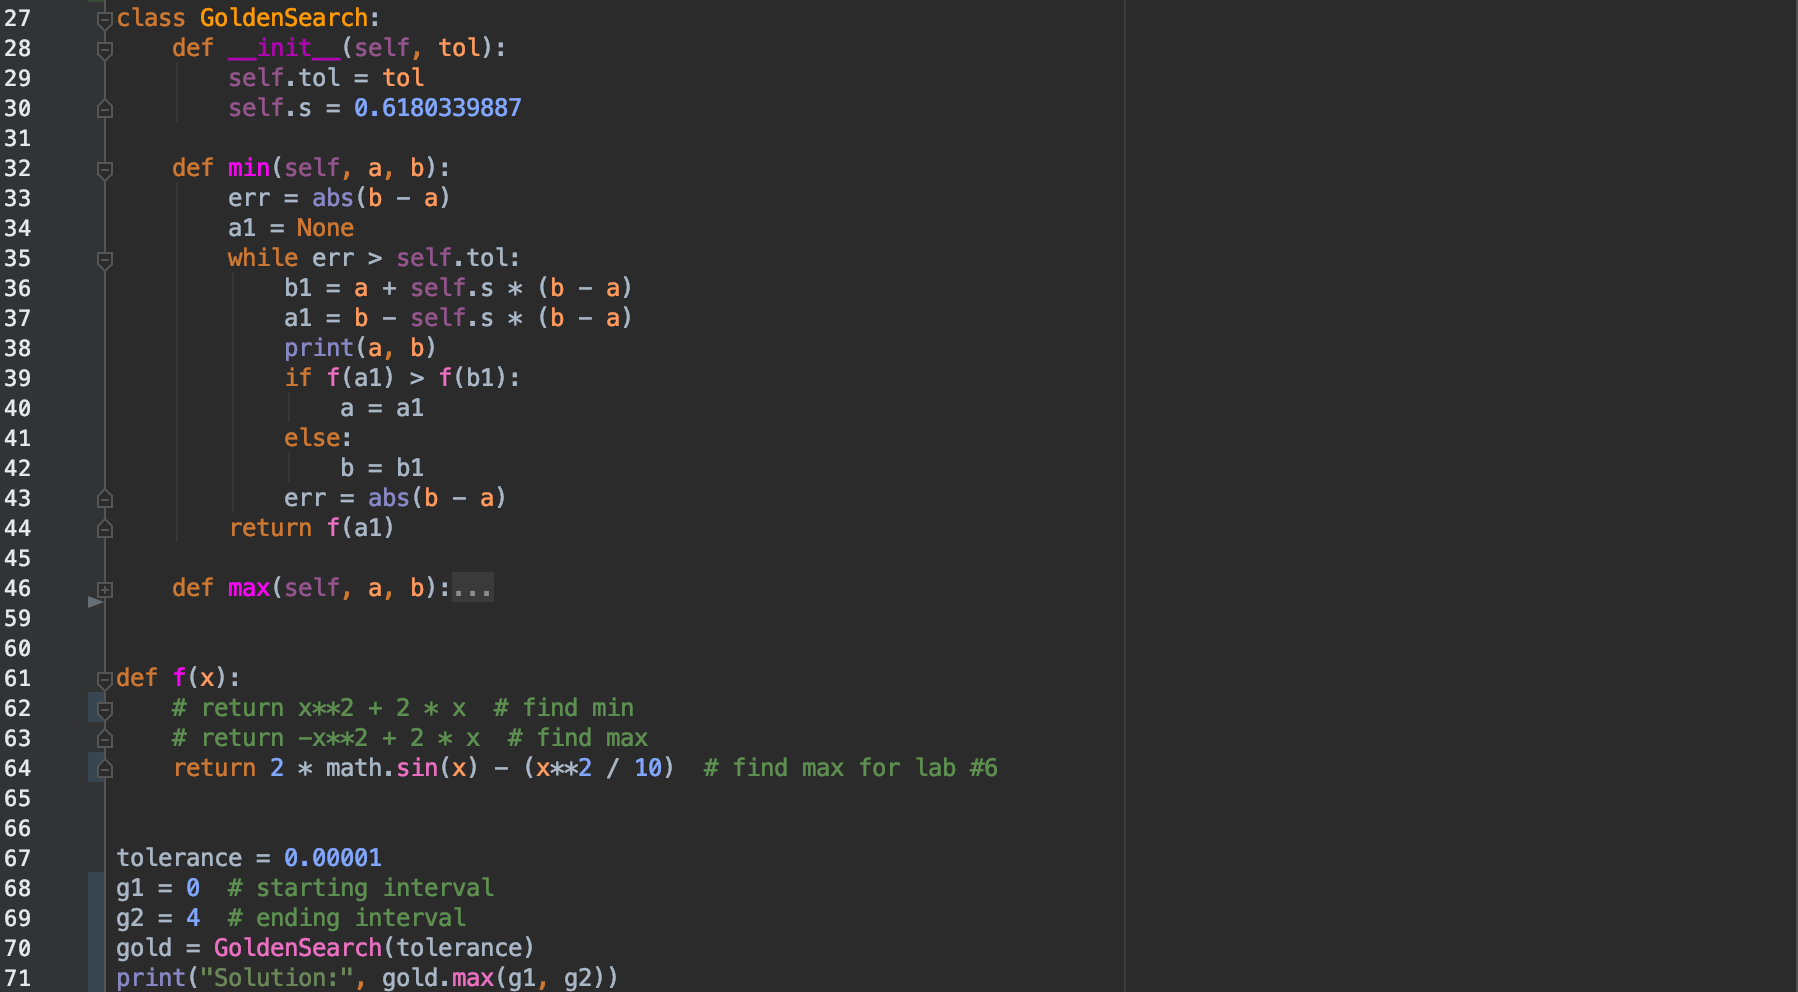
\includegraphics[width=1.0\linewidth]{PythonCode.png}
            		\end{figure}


\end{document}
